\setcounter{section}{4}

\Needspace{5\baselineskip}
\hypertarget{diffusion-forcingux4e0eroll-forcing}{%
\section{Diffusion Forcing与Roll Forcing}\label{diffusion-forcingux4e0eroll-forcing}}

\Needspace{5\baselineskip}
\hypertarget{ux4e00diffusion-forcing}{%
\subsection{一、Diffusion Forcing}\label{ux4e00diffusion-forcing}}

\Needspace{5\baselineskip}
\hypertarget{ux4e00ux95eeux9898ux80ccux666f-2}{%
\subsubsection{（一）问题背景}\label{ux4e00ux95eeux9898ux80ccux666f-2}}

传统序列建模主要有两种极端形式。

\begin{itemize}
\tightlist
\item
  下一个 Token 预测模型（Teacher Forcing）：例如 GPT 系列，支持生成可变长度序列，但它往往在连续数据（如视频生成）上由于误差累积容易导致预测崩溃，并且由于是逐步确定未来，无法根据未来的奖励或目标对当前步骤进行引导（Guidance）。
\item
  全序列扩散模型（Full-Sequence Diffusion）：常用于视频生成或离线强化学习规划。它将所有时间步作为一个整体添加相同水平的噪声，这虽然支持多步引导，但它采用了非因果架构，只能生成固定长度的序列，无法像人类一样基于因果不确定性来做决策。
\end{itemize}

目前大多扩散与自回归结合的模型都是分块生成，每次根据已经生成的块 \(x_1,\ldots,x_t\)，用扩散模型从噪声中生成新的一块 \(x_{t+1}\)。这里的隐含前提是，每一块的噪声水平相同。Diffusion Forcing 则不同，它为序列中的每一个 token 或每一块分配独立、随机的噪声水平，并训练一个因果模型来解掩码。

\Needspace{5\baselineskip}
\hypertarget{ux4e8cux8badux7ec3ux9636ux6bb5}{%
\subsubsection{（二）训练阶段}\label{ux4e8cux8badux7ec3ux9636ux6bb5}}

\Needspace{5\baselineskip}
Diffusion Forcing 的训练目标是让模型学会对具有任意且独立噪声水平的序列进行去噪。训练流程如下：

\begin{enumerate}
\def\labelenumi{\arabic{enumi}.}
\tightlist
\item
  从数据集中采样出真实观测序列 \((x_1,\ldots,x_T)\)。
\item
  分配独立噪声：遍历时间步 \(t=1,\ldots,T\)，为每一个 \(x_t\) 独立、均匀地采样一个噪声水平 \(k_t\in\{0,1,\ldots,K\}\)。
\item
  前向加噪：根据每个 token 对应的噪声水平进行前向扩散，得到观测值 \(x_t^{k_t}\)，并计算目标噪声 \(\epsilon_t\)。
\item
\Needspace{5\baselineskip}
  隐状态更新与噪声预测：模型根据前一时刻的隐状态 \(z_{t-1}\)、当前带噪观测 \(x_t^{k_t}\) 和噪声水平 \(k_t\)，预测噪声：
\end{enumerate}

\[
\hat{\epsilon}_t=\epsilon_\theta(z_{t-1},x_t^{k_t},k_t)
\]

同时更新新的状态 \(z_t\)。

\begin{enumerate}
\def\labelenumi{\arabic{enumi}.}
\setcounter{enumi}{4}
\tightlist
\item
  反向传播：将所有时间步的预测噪声与真实噪声计算均方误差（MSE Loss），并更新网络权重 \(\theta\)。
\end{enumerate}

\Needspace{5\baselineskip}
\hypertarget{ux4e09ux63a8ux7406ux9636ux6bb5ux57faux4e8eux6392ux7a0bux77e9ux9635ux7684ux63a7ux5236}{%
\subsubsection{（三）推理阶段：基于排程矩阵的控制}\label{ux4e09ux63a8ux7406ux9636ux6bb5ux57faux4e8eux6392ux7a0bux77e9ux9635ux7684ux63a7ux5236}}

\Needspace{5\baselineskip}
在算法定义中，排程矩阵 \(K\) 是一个维度为 \(M\times T\) 的二维网格：

\begin{itemize}
\tightlist
\item
  列（\(T\)）：代表序列的时间步长（Time steps），即 \(t\in\{1,2,\ldots,T\}\)。
\item
  行（\(M\)）：代表去噪采样的迭代步骤（Denoising steps），索引为 \(m\)。
\item
  元素数值 \(K_{m,t}\)：矩阵中的每一个元素 \(K_{m,t}\in\{0,1,\ldots,K\}\)，精确指定了第 \(t\) 个 token 在第 \(m\) 次去噪迭代时，所必须达到的目标噪声水平。其中 \(K\) 是纯白噪声，\(0\) 是干净数据。
\end{itemize}

\Needspace{5\baselineskip}
模型在推理时，会完全遵循这个矩阵的乐谱来演奏。具体流程如下：

\begin{enumerate}
\def\labelenumi{\arabic{enumi}.}
\tightlist
\item
  全局初始化：算法开始时，将整个目标序列 \(x_{1:T}\) 初始化为独立的高斯白噪声，此时所有 token 的噪声水平均是 \(K\)。
\item
  外层循环（按行降噪）：沿着矩阵的行向下遍历，例如从 \(M\) 减到 \(0\)。每一行代表一轮全局去噪刷新。
\item
  内层循环（因果推进）：在固定的行 \(m\) 内，沿着时间轴 \(t=1,\ldots,T\) 从左到右遍历。
\item
  目标读取与单步去噪：对于当前的 \((m,t)\)，算法读取矩阵设定值 \(k=K_{m,t}\)。随后，模型利用当前的隐状态 \(z_{t-1}\) 和带有当前实际噪声的 \(x_t\)，预测噪声 \(\epsilon_\theta(z_{t-1},x_t,k)\)，并通过 Langevin 动力学公式或 DDIM，将 \(x_t\) 的噪声精确降至目标层级 \(k\)。
\item
  因果状态更新：利用刚刚去噪后的 \(x_t\) 更新隐状态 \(z_t\)。由于是因果架构，这个更新后的 \(z_t\) 将包含 \(x_{1:t}\) 的最新信息，并传递给下一个时间步 \(t+1\)。
\end{enumerate}

\Needspace{5\baselineskip}
\hypertarget{ux56dbux57faux4e8eux6392ux7a0bux77e9ux9635ux7684ux751fux6210ux8303ux5f0f}{%
\subsubsection{（四）基于排程矩阵的生成范式}\label{ux56dbux57faux4e8eux6392ux7a0bux77e9ux9635ux7684ux751fux6210ux8303ux5f0f}}

基于排程矩阵 \(K\)，可以得到三种典型生成范式。

\hypertarget{ux5168ux5e8fux5217ux6269ux6563ux6a21ux5f0f}{%
\paragraph{1. 全序列扩散模式}\label{ux5168ux5e8fux5217ux6269ux6563ux6a21ux5f0f}}

如果我们要模仿传统视频扩散模型，如 SVD 或 Sora 的某一层逻辑，只需让矩阵的每一行元素完全相同。所有 token 同步均匀去噪。这接近传统的全序列扩散。

\hypertarget{ux81eaux56deux5f52ux6a21ux5f0f}{%
\paragraph{2. 自回归模式}\label{ux81eaux56deux5f52ux6a21ux5f0f}}

如果我们要模仿语言模型逐字生成，只需让矩阵呈现阶梯移动：确保前一个 token 和底噪降为 0 后，再开始生成下一个 token。这样既能保持因果顺序，又能保留扩散式局部细化。

\hypertarget{ux56e0ux679cux4e0dux786eux5b9aux6027ux6216ux91d1ux5b57ux5854ux6392ux7a0b}{%
\paragraph{3. 因果不确定性或金字塔排程}\label{ux56e0ux679cux4e0dux786eux5b9aux6027ux6216ux91d1ux5b57ux5854ux6392ux7a0b}}

这是论文的核心创新。它让矩阵呈现一种半金字塔或拉链状分布：让近期未来下降噪声较多，而远期未来保持较高噪声。控制原理是：当预测到 \(x_1\) 时，\(x_2\) 和 \(x_3\) 并没有完全成型，但它们携带了未来规划趋势的残影。这种安排完美地契合了贝叶斯滤波中对不确定世界中未来不确定性递增的建模，并允许现代尚未显现的信息平滑地反向传播回当前决策点，从而实现规划 Guidance。

\textbf{与 Transformer 架构的对应：}

在传统的自回归模型中，过去 token 一旦生成就固定死了，未来奖励无法修改过去的决定。而在 Diffusion Forcing 中，由于未来 token 虽然还处在较高噪声状态，但它们可以通过因果架构的隐状态 \(z_t\) 将梯度反向传播回较早的 token。这意味着模型可以``预见''远期未来的奖励，并在尚未完全固定的现在做出路径修正。

\Needspace{5\baselineskip}
这对应到 Transformer 注意力中，可以理解为两种机制：

\begin{enumerate}
\def\labelenumi{\arabic{enumi}.}
\tightlist
\item
  信息的彻底遮挡（DF 独有的 Fractional Masking）：如果我们改变排程矩阵，让未来 token 带有部分噪声，例如 \(k=K/2\)。此时，未来 token 变成了 \(\sqrt{\bar{\alpha}_k}x^0+\sqrt{1-\bar{\alpha}_k}\epsilon\)。它体内既含有真实的未来特征 \(x^0\)，又包含噪声。过去的 token 在计算自注意力时，可以从 \(V\) 矩阵中提取到被衰减过的未来信号。
\item
  当未来 token 被设为纯噪声时，它的 key 和 value 都接近随机噪声，注意力即使读到它，也不能获得真实信息，相当于传统 causal mask。
\end{enumerate}

通过控制未来 token 的噪声比例，Transformer 不需要改变任何网络结构，也不需要复杂的 attention mask 设计，就能实现从完全不因果到部分因果，再到严格因果的平滑过渡。

Diffusion Forcing 范式的优雅之处在于：噪声不再仅仅是需要被去除的障碍，而是变成了调节网络感受野、控制因果性以及传播规划梯度的核心控制介质。

\Needspace{5\baselineskip}
\hypertarget{ux4e94ux5229ux7528ux8499ux7279ux5361ux6d1bux5f15ux5bfcux5b9eux73b0ux89c4ux5212}{%
\subsubsection{（五）利用蒙特卡洛引导实现规划}\label{ux4e94ux5229ux7528ux8499ux7279ux5361ux6d1bux5f15ux5bfcux5b9eux73b0ux89c4ux5212}}

传统全序列扩散中，所有 token 处在相同噪声水平，当前和未来被绑定在同一条去噪轨迹上，很难在固定当前状态时采样多种未来。Diffusion Forcing 允许未来位置保持更高噪声，因此可以固定当前附近的状态，对未来噪声重复采样，得到多条可能轨迹。

\Needspace{5\baselineskip}
Monte-Carlo Guidance（MCG）在每次去噪时都采样未来。具体步骤如下：

\begin{enumerate}
\def\labelenumi{\arabic{enumi}.}
\tightlist
\item
  当前时刻的观测：智能体在环境的当前真实时间步，获得了历史积累的隐状态 \(z_{t-1}\)。
\item
  生成规划视距（Look-ahead Window）：模型并不会一口气规划到宇宙末日，而是设定一个向未来的视距 \(H\)。此时模型开始在隐空间中生成一个局部的未来序列 \(x_{t:t+H}\)。
\item
  每个去噪步的 MCG 采样：在这个局部序列 \(x_{t:t+H}\) 的每一次去噪迭代中，为了决定如何给当前的 \(x_t^k\) 去噪，模型都会在隐海中向未来 \(t+1\) 到 \(t+H\) 平行分叉出多条带有不确定性的轨迹。
\end{enumerate}

\Needspace{5\baselineskip}
计算这 \(N\) 条轨迹的预期未来奖励 \(R^{(i)}\)，并求平均值：

\[
\bar{R}(x_t^k)=\frac{1}{N}\sum_{i=1}^N R^{(i)}
\]

\Needspace{5\baselineskip}
然后对当前正在去噪的那个模糊输入 \(x_t^k\) 求偏导数（梯度）：

\[
\nabla_{x_t^k}\bar{R}(x_t^k)
\]

这个梯度代表着：如果想让当前带噪而模糊的 \(x_t^k\) 往梯度方向稍微挪动一点，那么它在未来演化出高奖励轨迹的概率就会最大化。

\Needspace{5\baselineskip}
随后，将未来奖励梯度直接注入到去噪预测中，类似于分类器引导（Classifier Guidance）的做法：

\[
\begin{aligned}
\tilde{\epsilon}
&=
\epsilon_\theta(x_t^k,k_t)
\\
&\quad -
\eta\sqrt{1-\bar{\alpha}_{k_t}}\nabla_{x_t^k}\bar{R}(x_t^k)
\end{aligned}
\]

然后使用这个被修正过的噪声 \(\tilde{\epsilon}\)，去把 \(x_t^k\) 降噪到下一个更清晰的层级 \(x_t^{k-1}\)。

在 MCG 中，被采样出来的 \(N\) 条未来轨迹在计算完梯度后会被直接丢弃。它们的作用只是充当临时侦察兵，为计算期望梯度（Expected Reward Gradient）提供方差更小的无偏估计。

经过多轮去噪，当前 token \(x_t\)，即当前需要执行的动作 \(\hat{u}_t\)，会被清晰化。智能体在现实中只执行这个动作，并将环境返回的真实奖励 \(r_t\) 和下一个观测 \(o_{t+1}\) 继续用于下一轮滚动规划。这与 MPC（Model Predictive Control）思想一致。

通过这种方式，当前动作在从纯噪声降为 0 的漫长过程中，每走一步，都会受到未来预期梯度的拉扯。最终，当它降噪为 0 时，它本身就已经是一条通向最优解的动作。这种方法不仅采样效率极高，而且生成的轨迹更加平滑且符合物理规律。

\Needspace{5\baselineskip}
\hypertarget{ux516dux4e3aux4ec0ux4e48ux4f20ux7edfux81eaux56deux5f52ux548cux6269ux6563ux6a21ux578bux90fdux65e0ux6cd5ux5c06ux672aux6765ux68afux5ea6ux4f20ux5230ux8fc7ux53bbux800cux8be5ux67b6ux6784ux53efux4ee5}{%
\subsubsection{（六）为什么传统自回归和扩散模型都无法将未来梯度传到过去，而该架构可以？}\label{ux516dux4e3aux4ec0ux4e48ux4f20ux7edfux81eaux56deux5f52ux548cux6269ux6563ux6a21ux578bux90fdux65e0ux6cd5ux5c06ux672aux6765ux68afux5ea6ux4f20ux5230ux8fc7ux53bbux800cux8be5ux67b6ux6784ux53efux4ee5}}

自回归的瓶颈是过早做硬承诺。自回归模型必须把当前 token 先完全确定下来，例如划分布采样、argmax 或温度采样，才能将它作为历史条件输入进去，从而推演未来 \(x_{t+1}\)。一旦已经被硬确认，当前状态就结束了，当然无法让未来奖励对它做梯度更新。

纯扩散的瓶颈是无法产生分支。在全序列扩散中，如果固定了当前的带噪状态 \(x_t^k\)，并且大家都在同一个噪声层级上继续去噪，整个计算图就固定了。你只能得到一条确定的、和当前状态紧紧绑定的未来轨迹。轨迹方差极大时，这个梯度还可能非常不稳定。

\Needspace{5\baselineskip}
Diffusion Forcing 的优势是同时保留未来不确定性和当前可导性：

\begin{enumerate}
\def\labelenumi{\arabic{enumi}.}
\tightlist
\item
  未来的噪声水平较高，远远高于当下的噪声水平。这意味着未来还没有被锁定，我们可以把当前的 \(x_t^k\) 冻住，然后向未来注入成百上千个不同的纯白噪声，生成足够多的未来分支。
\item
  当下的 token 并没有像自回归模型那样被硬确认，而仍然处于一个微弱的噪声状态，例如 \(k=2\)。因为它还是一个连续的、带有不确定性的变量，奖励期望梯度可以直接作用于它，平滑地修改它在进一步 Langevin 动力学中的去噪方向。
\end{enumerate}

\Needspace{5\baselineskip}
\hypertarget{ux4e03ux5386ux53f2ux4fe1ux606fux8f7bux5faeux52a0ux566aux6280ux5de7}{%
\subsubsection{（七）历史信息轻微加噪技巧}\label{ux4e03ux5386ux53f2ux4fe1ux606fux8f7bux5faeux52a0ux566aux6280ux5de7}}

在需要超长序列生成时，Diffusion Forcing 利用采样阶段的灵活性提出了一个极其聪明的技巧，防止误差累积：为历史信息轻微加噪。

在生成下一帧 \(x_t\) 时，DF 并不完全信任上一帧 \(x_{t-1}\)。因为它是模型自己生成的，必定含有微小瑕疵。相反，DF 会保留一个带有极其微小噪声 \(k_{\mathrm{small}}\) 的上一帧隐状态 \(z_{t-1}\)，例如 \(K_{\mathrm{small}}\ll K\)，并以此为条件生成下一帧。由于模型在训练时本身就是基于带噪输入学习的，这使得自回归生成一直处于分布内（in-distribution），从而实现了无限长度的稳定 rollout，彻底解决了传统 Teacher Forcing 模型的崩溃问题。

\Needspace{5\baselineskip}
\hypertarget{ux516bux7406ux8bbaux53efux884cux6027ux8bc1ux660e}{%
\subsubsection{（八）理论可行性证明}\label{ux516bux7406ux8bbaux53efux884cux6027ux8bc1ux660e}}

从理论上看，论文附录 A 给出了一套基于证据下界（ELBO）的严格数学证明。模型实际上是在优化一个修改版的带权 ELBO。假设前向马尔可夫过程为 \(q(x^{1:K}|x^0)=\prod_{k=1}^K q(x^k|x^{k-1})\)，生成模型参数化为 \(p_\theta\)。作者证明，DF 的训练过程最大化了真实联合分布对数似然的下界。

\Needspace{5\baselineskip}
根据定理 A.1，对于随机独立采样的噪声水平 \(k_{1:T}\)，其期望对数似然的 ELBO 可以写为：

\[
\begin{aligned}
&\mathbb{E}_{\mathrm{forward}}
\left[
\log p_\theta\left((x_t^k)_{1\le t\le T}\right)
\right] \\
&\quad \ge \mathcal{C}(x_{1:T}^0)
+\mathbb{E}_{\mathrm{forward},p_\theta,z_{1:T}}
\left[
\sum_{t=1}^T
\right. \\
&\qquad \left.
\left(
\frac{1}{K+1}\log p_\theta(x_t^0\mid z_{1:t},z_{t-1})
+\sum_{j=2}^K\frac{j}{K+1}
\right.
\right. \\
&\qquad\qquad \left.\left.
{}\cdot D_{\mathrm{KL}}\left(
q(x_t^{j-1}\mid x_t^j,x_t^0)
\middle\|
p_\theta(x_t^{j-1}\mid x_t^j,z_{t-1})
\right)
\right)
\right]
\end{aligned}
\]

\Needspace{5\baselineskip}
这里的核心发现是：在隐变量 \(z_{t-1}\) 完全表达力足够的情况下，由于各时间步 \(t\) 上的损失项是解耦的，权重项 \(\frac{j}{K+1}\) 可以被忽略或重新加权。最终，训练目标简化为熟悉的扩散模型最小二乘形式：

\[
\mathcal{L}(\theta)=
\mathbb{E}_{k_{1:T},x,\epsilon}
\left[
\sum_{t=1}^T
\left\|
\epsilon_t-\epsilon_\theta(z_{t-1},x_t^{k_t},k_t)
\right\|^2
\right]
\]

由于损失覆盖了序列中所有可能的局部掩码排列，这保证了在推理时，模型可以用任意的时间步调度策略来采样真实数据的子序列边缘分布。

\Needspace{5\baselineskip}
\hypertarget{ux4e8crolling-forcingux6edaux52a8ux53bbux566aux751fux6210}{%
\subsection{二、Rolling Forcing：滚动去噪生成}\label{ux4e8crolling-forcingux6edaux52a8ux53bbux566aux751fux6210}}

对于长视频的流式生成，Self Forcing 的确解决了训练和推理的不匹配问题，但并没有完全解决误差累积的问题。Rolling Forcing 旨在解决此问题。

\begin{enumerate}
\def\labelenumi{\arabic{enumi}.}
\tightlist
\item
  \textbf{滑动窗口联合去噪}：不再逐帧去噪，而是在一个滑动窗口内进行联合去噪。窗口内的 \(T\) 帧被赋予递增的噪声等级，从几乎清晰到完全噪声。在窗口内部，模型通过双向注意力机制，让相对清晰的帧帮助指导噪声严重的帧去噪，在误差传播到下一帧之前，就在局部窗口内将其扼杀。每一次前向传播，模型只输出窗口中最清晰的一帧，然后窗口整体前移。
\end{enumerate}

\begin{figure}[htbp]
\centering
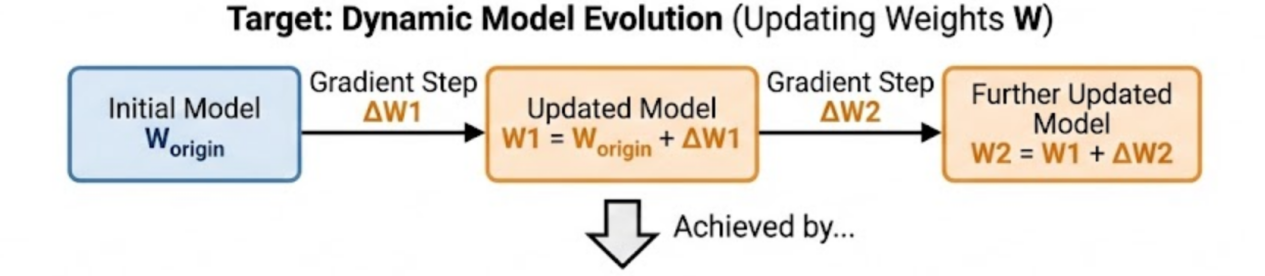
\includegraphics{images/image-0044.png}
\caption{Diffusion Forcing 与 Rolling Forcing 的序列生成方式对比}
\end{figure}

\begin{figure}[htbp]
\centering
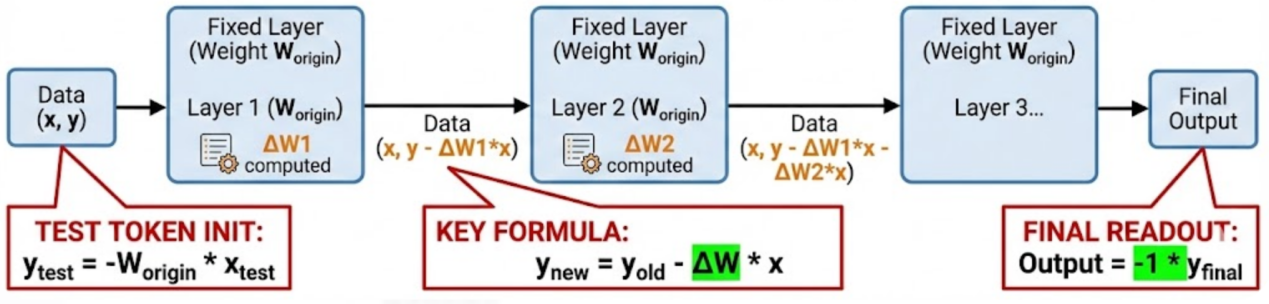
\includegraphics{images/image-0045.png}
\caption{图中颜色和注意力连线的含义}
\end{figure}

\begin{enumerate}
\def\labelenumi{\arabic{enumi}.}
\setcounter{enumi}{1}
\item
  \textbf{Attention Sink}：将视频最开始几帧的 Key-Value 状态缓存下来，作为``全局上下文锚点''，确保模型无论生成到多远，都能回看到视频的初始状态，从而极大地保证全局风格、色调等信息的一致性。
\item
  \textbf{混合训练策略}：将 RF 的滚动窗口目标与 SF 的逐帧生成目标混合训练。SF 的目标在此处起到了正则化作用，防止滚动窗口机制导致不自然的相机运镜。
\end{enumerate}

\FloatBarrier
\Needspace{5\baselineskip}
\hypertarget{ux53c2ux8003ux6587ux732e-142}{%
\subsection{参考文献}\label{ux53c2ux8003ux6587ux732e-142}}

\vspace{0.25em}
\begin{itemize}
\tightlist
\item
  Chen, B., Monso, D. M., Du, Y., Simchowitz, M., Tedrake, R., \& Sitzmann, V. (2024). \href{https://arxiv.org/abs/2407.01392}{Diffusion Forcing: Next-token Prediction Meets Full-Sequence Diffusion}. NeurIPS.
\item
  Liu, K., Hu, W., Xu, J., Shan, Y., \& Lu, S. (2025). \href{https://arxiv.org/abs/2509.25161}{Rolling Forcing: Autoregressive Long Video Diffusion in Real Time}. ICLR.
\end{itemize}

\clearpage
